\documentclass[fontsize = 10pt, paper= a4,twocolumn,column_gap=5zw]{jlreq}

\usepackage[dvipdfmx]{graphicx}
\usepackage{color}
\usepackage{listings}
\usepackage{url}
\definecolor{OliveGreen}{rgb}{0.0,0.6,0.0}
\definecolor{Magenta}{cmyk}{0, 1, 0, 0}
\definecolor{colFunc}{rgb}{1,0.07,0.54}
\definecolor{CadetBlue}{cmyk}{0.62,0.57,0.23,0}
\definecolor{Brown}{cmyk}{0,0.81,1,0.60}
\definecolor{colID}{rgb}{0.63,0.44,0}
\lstset{
language={C},                   %言語の指定
basicstyle={\ttfamily\small},        %書体の指定
backgroundcolor={\color[gray]{.95}}, %背景色と透過度
keywordstyle={\color{blue}},         %キーワード(int, ifなど)の書体指定
commentstyle={\color{OliveGreen}},   %注釈の書体 
stringstyle=\color{Magenta},         %文字列
frame=single,                        %枠縁(leftline,topline,bottomline,lines,trBL,shadowbox, single)
numbers=left,                        %行番号表示
numberstyle={\ttfamily\small},       %行番号の書体指定
breaklines=true,                     %折り返し(自動改行)
breakindent = 10pt,                  %自動改行後のインデント量(デフォルトでは20[pt])	
tabsize=2,                           %タブの大きさ
captionpos=t                         %キャプションの場所(t,b : "tb"ならば上下両方に記載)
}
\renewcommand{\lstlistingname}{図} % キャプション名の指定

\begin{document}

\title{統計分析法 第7週レポート}
\author{202212022 田島瑞起}
\date{2023/12/05}
\maketitle
\section{設問1-1}
    A,Bについてのヒストグラムを下記の図で示す。
    \begin{figure}
        \centering
        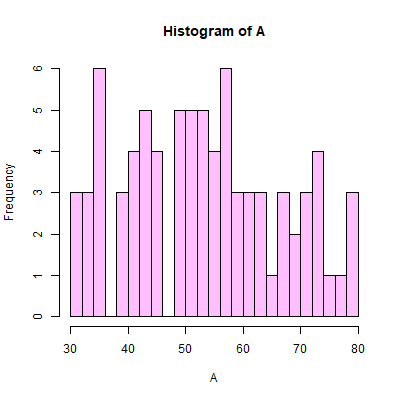
\includegraphics[width=4cm]{7-1-1.png}
    \end{figure}
    \begin{figure}
        \centering
        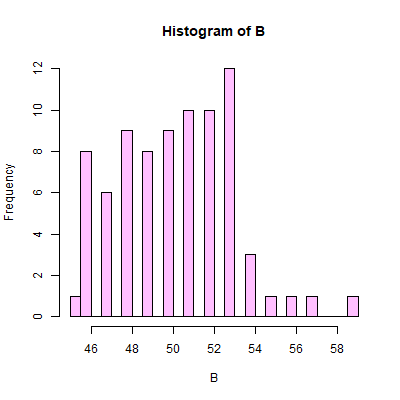
\includegraphics[width=4cm]{7-1-2.png}
    \end{figure}

\section{設問1-2}
    今回得られたA群B群の平均値差の実測値は,2.87である。
    A群B群をブートストラップ処理し,二群間の平均値差の理想分布を図示し,実測値を添付した結果,下記の図となった。
    \begin{figure}
        \centering
        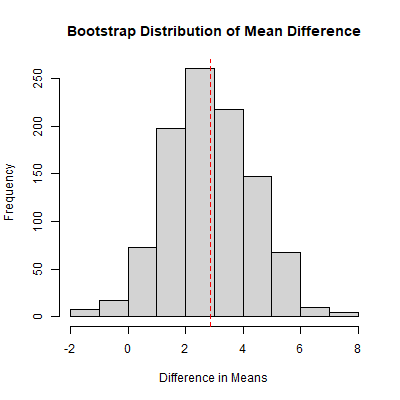
\includegraphics[width=4cm]{7-1-3.png}
    \end{figure}

\section{設問1-3}
    今回の帰無仮説は「A,B群に平均値の差がない」を設定し,有意水準を両側検定の為0.10に設定する。
    ブートストラップ処理を実行し,両側検定のp値を求めるとp=0.976と表示された。
    これは有意水準を大きく上回る値であるため,帰無仮説を棄却することは出来ない。
    よってA,B群の平均値に差がないと言うことが出来る。

\section{設問1-4}
    t-testを用いて今回のデータセットについて検証したところ下記の結果が表示された。
    ブートストラップ処理とは結果が大きく異なる。
    この際考えられる要因としては,t検定では正規分布を仮定した検証方法であるため,
    データの非対称性や外れ値に敏感に反応してしまう可能性がある。
    これに対して復元抽出して理想分布を作成するブートストラップ処理では,非対称性や外れ値に強い
    ロバストな手法であるため,t-検定よりも大きなp値を示したと考えられる。
    \begin{lstlisting}[basicstyle=\ttfamily\footnotesize, frame=single, caption=s2212022-1.c ,label=s2212022-1.c]
        Welch Two Sample t-test

        data:  A and B
        t = 1.8629, df = 86.06, p-value = 0.06589
        alternative hypothesis: true difference in means is not equal to 0
        95 percent confidence interval:
         -0.1923156  5.9231156
        sample estimates:
        mean of x mean of y 
          53.1654   50.3000 
        \end{lstlisting}

\section{設問1 ソースコード}
\begin{lstlisting}[basicstyle=\ttfamily\footnotesize, frame=single, caption=s2212022-1.c ,label=s2212022-1.c]
    #課題1-1
    setwd('Z:/stats_work')
    ReadData <- read.table('data_p.txt')
    A <- ReadData$V1
    B <- ReadData$V2
    A <- A[2:length(A)]
    B <- B[2:length(B)]
    A <- as.numeric(A)
    B <- as.numeric(B)
    png("7-1-1.png", width = 400, height = 400)
    hist(A,breaks=20,col='#ff00ff40')
    dev.off()
    png("7-1-2.png", width = 400, height = 400)
    hist(B,breaks=20,col='#ff00ff40')
    dev.off()
    
    #課題1-2,1-3
    
    # ライブラリの読み込み
    library(boot)
    
    # データの読み込み
    setwd('Z:/stats_work')
    ReadData <- read.table('data_p.txt')
    A <- as.numeric(ReadData$V1[-1])
    B <- as.numeric(ReadData$V2[-1])
    
    # ブートストラップサンプリング関数
    bootstrap_function <- function(data, indices) {
      sample_A <- data$A[indices]
      sample_B <- data$B[indices]
      diff_mean <- mean(sample_A) - mean(sample_B)
      return(diff_mean)
    }
    
    # オリジナルデータ
    obs_diff_mean <- mean(A) - mean(B)
    
    # ブートストラップ法
    set.seed(22)  # 再現性のためにシードを設定
    bootstrap_results <- boot(data.frame(A, B), statistic = bootstrap_function, R = 1000)
    
    # ブートストラップ結果からp値の計算
    p_value <- 2 * min(mean(bootstrap_results$t >= obs_diff_mean), mean(bootstrap_results$t <= obs_diff_mean))
    
    # ブートストラップ結果のヒストグラム(理論分布)
    png("7-1-3.png", width = 400, height = 400)
    hist(bootstrap_results$t, main = "Bootstrap Distribution of Mean Difference", xlab = "Difference in Means")
    abline(v = obs_diff_mean, col = "red", lty = 2)  # オリジナルデータの平均差
    dev.off()
    
    # p値の表示
    cat("Observed Difference in Means:", obs_diff_mean, "\n")
    cat("Bootstrap p-value:", p_value, "\n")
    
    #課題1-4
    t.test(A, B)
    \end{lstlisting}

\section{設問2-1}
乱数の個数に応じた円周率の近似結果をモンテカルロシュミレーションで実行し,個数に応じた近似値をプロットした結果下記の図の通りとなった。
\begin{figure}
    \centering
    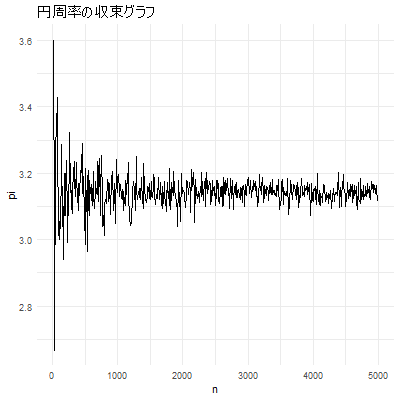
\includegraphics[width=4cm]{7-2-1.png}
\end{figure}

\section{設問2-2}
乱数の個数に応じた円周率の近似結果をモンテカルロシュミレーションで乱数の個数ごとに100回円周率を近似し,その100回で得られた円周率の平均値と分散を,乱数の個数に応じてプロットした結果下記の図の通りとなった。
\begin{figure}
    \centering
    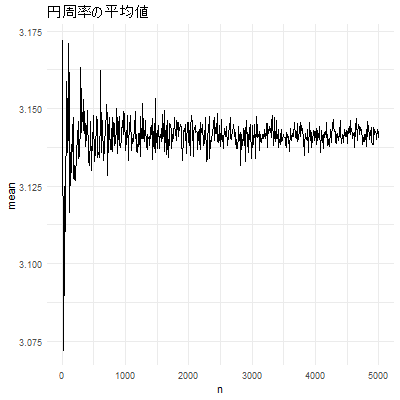
\includegraphics[width=4cm]{7-2-2.png}
\end{figure}

\begin{figure}
    \centering
    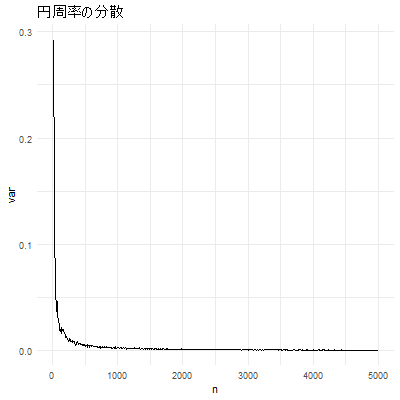
\includegraphics[width=4cm]{7-2-3.png}
\end{figure}

\section{設問2-3}
設問2-1の結果よりkの値が大きくなれば正確な円周率の値に収束する。設問2-2の結果よりkの値が大きくなれば円周率の平均値は正確な円周率の値に収束し,分散は0に収束する。

\section{設問1 ソースコード}
\begin{lstlisting}[basicstyle=\ttfamily\footnotesize, frame=single, caption=s2212022-1.c ,label=s2212022-1.c]
    #課題2-1

    estimate_pi <- function(num_samples) {
      # ランダムに点をサンプリング
      x <- runif(num_samples, -1, 1)
      y <- runif(num_samples, -1, 1)
      # 円内に入る点の数を数える
      inside_circle <- x^2 + y^2 <= 1
      num_inside <- sum(inside_circle)
      # 円周率の推定値を計算
      pi_estimate <- 4 * (num_inside / num_samples)
      
      return(pi_estimate)
    }
    
    # サンプル数を指定して円周率を求める
    n_array <- seq(10,5000,10)
    pi_array <- numeric(length(n_array))
    for( k in n_array){
        i <- k / 10
        pi_array[i] <- estimate_pi(k)
    }
    
    install.packages("ggplot2")
    # ライブラリの読み込み
    library(ggplot2)
    # グラフの作成
    df <- data.frame(n = n_array, pi = pi_array)
    # 折れ線グラフの描画
    png("7-2-1.png",width=400,height=400)
    ggplot(df, aes(x = n, y = pi)) +
      geom_line() +
      labs(title = "円周率の収束グラフ",
           x = "n",
           y = "pi") +
      theme_minimal()
    dev.off()
    
    #課題2-2
    pi_mean_array <- numeric(length(n_array))
    pi_var_array <- numeric(length(n_array))
    r <- 100
    
    for( k in n_array){
        pi_array_tmp <- numeric(100)
        i <- k / 10
        for( j in 1:r){
            pi_array_tmp[j] <- estimate_pi(k)
        }
        pi_mean_array[i] <- mean(pi_array_tmp)
        pi_var_array[i] <- var(pi_array_tmp)
    }
    
    # グラフの作成
    df <- data.frame(n = n_array, mean = pi_mean_array)
    # 折れ線グラフの描画
    png("7-2-2.png",width=400,height=400)
    ggplot(df, aes(x = n, y = mean)) +
      geom_line() +
      labs(title = "円周率の平均値",
           x = "n",
           y = "mean") +
      theme_minimal()
    dev.off()
    
    # グラフの作成
    df <- data.frame(n = n_array, var = pi_var_array)
    # 折れ線グラフの描画
    png("7-2-3.png",width=400,height=400)
    ggplot(df, aes(x = n, y = var)) +
      geom_line() +
      labs(title = "円周率の分散",
           x = "n",
           y = "var") +
      theme_minimal()
    dev.off()
    \end{lstlisting}
\end{document}